\section{Representation and cut-geometry diagnostics}\label{sec:oracle}
A point tangent depends on the algebraic representation of a feasible set. A radial boundary construction has a restricted invariance when its anchor is held fixed. The relationship between ESH and cutting planes for gauge reformulations is already established \citep{serrano2020}; the results here isolate consequences that can be checked by the actual separator without a full GDP solve.

\subsection{Equivalent rows and fixed-anchor invariance}
\begin{proposition}[Boundary halfspace invariance]\label{prop:invariance}
Let $g$ be convex and differentiable on a neighborhood of its box, and let $\phi$ be convex, differentiable and strictly increasing on an interval containing the values of $g$, with $\phi(0)=0$ and $\phi'(0)>0$. The row $\widehat g=\phi\circ g\le0$ defines the same feasible set and is convex. For a fixed strict anchor and exterior point, exact rowwise ESH gives the same halfspace for $g$ and $\widehat g$, including after the hull transform. At an exterior point $p$ with $v=g(p)>0$ and $\phi'(v)>0$, the ECP inequality for $\widehat g$ is
\begin{equation}\label{eq:reexpressed-ecp}
 \nabla g(p)^T(x-p)\le-\frac{\phi(v)}{\phi'(v)},
\end{equation}
instead of the right side $-v$ for $g$.
\end{proposition}
\begin{proof}
Strict monotonicity and $\phi(0)=0$ preserve the signs of all row values. Convexity of $g$, monotonicity of $\phi$ and convexity of $\phi$, in that order, prove convexity of the composition. The common segment has the same boundary point $z$ for both rows. At it, $\nabla\widehat g(z)=\phi'(0)\nabla g(z)$ and both row values vanish. The affine coefficients, including the homogeneous perspective coefficients, are therefore multiplied by the same positive factor. At $p$, the chain rule gives tangent
$\phi(v)+\phi'(v)\nabla g(p)^T(x-p)\le0$; division by $\phi'(v)>0$ proves \eqref{eq:reexpressed-ecp}.
\end{proof}
A positive linear $\phi$ preserves point tangents too, but a general convex increasing transformation does not. Convexity implies $\phi(v)\le v\phi'(v)$ for $v>0$, so under this transformation the ECP inequality at the \emph{same} exterior point is no stronger than the original one. This does not compare subsequent master trajectories or runtime. The proposition requires the same anchor: the auxiliary interior optimization itself can respond to a changed representation. It also requires exact boundary roots. Approximate root tolerances, row scaling and finite arithmetic need not preserve the halfspace.

\subsection{A scalar recurrence and its interpretation}
\begin{proposition}[An arbitrarily long point-tangent transient]\label{prop:scalar}
For $a\ge2$, consider
\begin{equation}\label{eq:scalar}
 \min\{-x:0\le x\le2,\quad g_a(x)=\exp(a(x-1))-1\le0\}.
\end{equation}
Every instance has feasible interval $[0,1]$, optimum $-1$, and strict anchor zero. Starting from the box alone, or the box plus a tangent at zero, the first master optimum is $p_0=2$. One exact ESH cut gives $x\le1$. With exact ECP and all cuts retained, successive master optima satisfy
\begin{equation}\label{eq:scalar-recurrence}
 p_{k+1}=p_k-\frac{1-\exp[-a(p_k-1)]}{a},\qquad p_k>1.
\end{equation}
For any fixed $0<\eta<1$, reaching $p_k\le1+\eta$ requires $k>a(1-\eta)$ cuts. Nevertheless $p_k\downarrow1$.
\end{proposition}
\begin{proof}
The anchor tangent gives $x\le(e^a-1)/a$, whose right side exceeds two for $a\ge2$: $e^2>5$, and the derivative of $e^a-1-2a$ is positive for $a\ge2$. It thus leaves the box optimum unchanged. The segment from zero to any $p>1$ meets the unique boundary at $z=1$, where $g_a'(1)=a>0$; ESH gives $a(x-1)\le0$. The ECP tangent at $p_k$ yields
\[
 x\le p_k-\frac{g_a(p_k)}{g_a'(p_k)}
 =p_k-\frac{1-\exp[-a(p_k-1)]}{a}.
\]
For $u>0$, $0<1-e^{-u}<u$. Therefore this new bound is strictly between one and $p_k$, and all older upper bounds are weaker. This proves the recurrence for the actual master optima, rather than merely for a proposed iteration. Each decrease is strictly less than $1/a$, so $2-p_k<k/a$. If $p_k\le1+\eta$, then $1-\eta\le2-p_k<k/a$, proving the lower bound. Monotonicity and the lower bound one give a limit $p_*\ge1$; if $p_*>1$, continuity in the recurrence gives a strictly positive limiting decrement, a contradiction.
\end{proof}
Equation~\eqref{eq:scalar-recurrence} is precisely Newton's method for the equation $g_a(x)=0$, started from the exterior point. The example exhibits a representation-dependent initial transient, not a failure of asymptotic Newton convergence: with $e_k=p_k-1\to0$, Taylor expansion gives
\[
 e_{k+1}=\tfrac{a}{2}e_k^2+O(e_k^3)\quad\text{for fixed }a.
\]
This elementary mechanism is not GDP-specific. Nor is the iteration lower bound a runtime lower bound: ESH spends additional row evaluations on its boundary search. Large $a$ creates conditioning and overflow concerns in finite arithmetic. A transformed function-residual tolerance is not a common geometric accuracy criterion across $a$; a numerical diagnostic should instead use $\max\{0,p_k-1\}$, which is also the objective error here, and count evaluations.

\subsection{Centered geometry and explicit non-dominance}
For the centered ellipsoid row $q(x)=x^TQx-1$, $Q\succ0$, take anchor zero and $p=rQ^{-1/2}u$ with $r>1$ and $\|u\|_2=1$. The boundary is $z=Q^{-1/2}u$. ESH gives $z^TQx\le1$, whereas ECP gives
\[
 z^TQx\le\frac{r^2+1}{2r}=1+\frac{(r-1)^2}{2r}>1.
\]
Thus ESH dominates for this centered geometry. A convex increasing representation change as in \cref{prop:invariance} preserves the ESH halfspace and weakens or preserves the exterior-point tangent. This accounts for the selected centered diagnostic cases; it is not a general dominance statement.

\begin{example}[Neither policy generally dominates]\label{ex:nondominance}
Let $g(x_1,x_2)=x_1^2+x_2^2-1$ on $[-2,2]^2$, $p=(2,0)$ and $\bar x=(0,9/10)$. ECP gives $x_1\le5/4$. Solving the segment-circle intersection yields
\[
 z_1=\frac{162+20\sqrt{157}}{481},\qquad
 z_2=\frac9{10}-\frac9{20}z_1,
 \qquad z_1^2+z_2^2=1,
\]
and ESH gives $z_1x_1+z_2x_2\le1$. Direct bounds on the square root give $0.85<z_1<0.87$ and $0.50<z_2<0.52$. The point $(1.2,1)$ satisfies ECP, but its ESH left side exceeds $1.2(0.85)+0.50=1.52>1$. The point $(1.3,-2)$ violates ECP, but its ESH left side is less than $1.3(0.87)-2(0.50)=0.131<1$. Both witnesses belong to the common box. Consequently neither halfspace contains the other. They are witnesses about the outer approximations, not feasible disk points. Setting $\lambda=1$ transfers this non-dominance to the perspective cuts.
\end{example}
These examples explain why cut count, cut depth at one candidate and total solver benefit must be measured separately. They justify a controlled experiment without assuming which policy must win.

% Stage 3 owns the empirical diagnostic subsection below this marker.
% It must preserve the theory above and report frozen scalar/ellipsoid records,
% analytic oracle wrappers, evaluation counts, stopping criteria and scope.

\subsection{Evaluation of the frozen separator}\label{sec:oracle-empirical}
A solver-free experiment invokes the actual frozen \texttt{LBESH.\_esh\_cuts} routine with counted analytic value/gradient wrappers and the actual nonlinear-row container. It evaluates the cut algorithm, not the Pyomo/SymPy expression compiler. Exponential wrappers use \texttt{expm1} for stable evaluation. The anchor is prescribed, no GDP or optimization subproblem is solved, and every ESH call is checked to exclude ECP fallback. Both cut and feasibility tolerances are $10^{-12}$; bisection stops at a parameter-bracket width below $10^{-10}$.

For the scalar example, the initial master is the box alone for every representation, including $a=1$. The base row $x-1$ is also passed through the separator; a real model extractor would instead recognize it as affine. After each cut its floating-point coefficients update the scalar upper bound by direct division. All cases stop at the common geometric criterion $(x-1)_+\le10^{-8}$, rather than a representation-dependent function residual. \Cref{tab:oracle,fig:oracle-cost} show the complete design. ECP uses 1, 5, 6, 8, 12, 20 and 36 cuts for the base row and $a=1,2,4,8,16,32$; ESH uses one throughout. Each ECP cut requires two value calls and one gradient; each ESH cut requires 37 values and one gradient, including 34 bisection evaluations and one value each at the candidate, anchor and tangent point. Bisection does not stop early at an exact zero. Thus ESH uses more total value calls through $a=8$, despite using fewer cuts. Scalar ESH bounds equal one at recorded precision; ECP's largest terminal geometric error is $2.56\cdot10^{-11}$ and recurrence disagreement is at most $2.23\cdot10^{-16}$.
\begin{figure}[tb]
\centering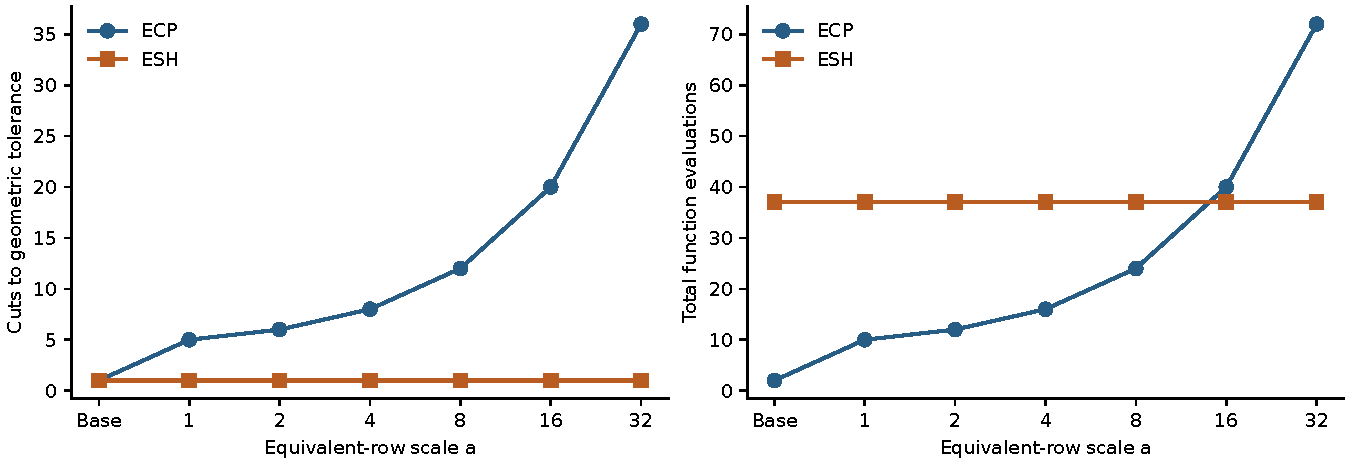
\includegraphics[width=\linewidth]{figures/oracle_cost.pdf}
\caption{Scalar representation diagnostic using the frozen separator. Fewer cuts do not imply fewer function evaluations. The design fixes the anchor and uses the same geometric stopping tolerance for every equivalent row.}\label{fig:oracle-cost}
\end{figure}

The two-dimensional design uses $Q=I$ or $\operatorname{diag}(1,4)$, anchor zero, and $p=rQ^{-1/2}(\cos\theta,\sin\theta)$ with $r\in\{1.25,1.75\}$ and $\theta=2\pi k/16$, $k=0,\ldots,15$. Both policies are tested on the base row $q(x)=x^TQx-1$ and the six transformed rows $\exp(aq(x))-1$ with $a\in\{1,2,4,8,16,32\}$, giving $2\cdot2\cdot16\cdot7\cdot2=896$ individual cuts. Every point lies in $[-2,2]^2$. After unit-normal scaling, ESH support constants differ from the analytic supporting constants by at most $4.45\cdot10^{-16}$; normal errors are below $10^{-12}$. ECP constants differ from their own analytic ECP constants by less than $10^{-9}$; these constants generally differ from the ellipsoid's supporting constants. Each cut $n^Tx+c\le0$ passes the analytic ellipsoid support check $\sqrt{n^TQ^{-1}n}+c\le10^{-10}$. These floating-point comparisons do not constitute interval certificates.

At the disk point $(1.75,0)$, ESH depth is 0.75 for every representation; ECP depth falls from 0.589286 for the base row to 0.008929 for $a=32$. This invariance is numerical evidence for this fixed centered geometry, where the two normals are parallel. The off-center control from the preceding subsection yields ESH depth 0.715590 versus ECP's 0.75, and reproduces both non-containment witnesses. It prevents the centered examples from suggesting uniform cut dominance.

Nine timing samples are retained for every scalar sequence and two-dimensional cut. Scalar median times range approximately 41--85 microseconds for ESH and 10--533 microseconds for ECP across representations. They exclude imports and creation of the counted function and oracle objects, but include oracle calls, per-call row/container construction and Python bookkeeping. At these durations, concurrent work and measurement overhead preclude a robust speed interpretation. There are no MILP, NLP or anchor-computation costs here. The diagnostic establishes a representation-sensitive mechanism and its oracle cost; it does not show that this mechanism explains every GDP outcome.
